\section{Calcolo preventivo delle env map}
\label{sec:chapter_lrl_calcolo_preventivo_env}

Le env-map nel presente lavoro di tesi sono risultate essenziali per permettere la creazioni di effetti di riflessione e rifrazione che non appesantissero eccessivamente il carico di lavoro del ciclo di render. 
L’utilizzo di esse al posto dei normali specchi in Three.js, come spiegato durante l’introduzione, ha permesso la computazione di scene con molti effetti di riflessione/rifrazione anche in ambienti browser; cosa che altrimenti sarebbe stata impossibile da realizzare.
Nel presente lavoro di tesi le env-map sono create utilizzando Three.js in quanto ne permette la facile creazione tramite l’utilizzo di un oggetto \texttt{CubeCamera}.
L’oggetto CubeCamera è composto da sei camere con volume prospettico centrate al suo interno, ogni camera è orientata verso una diversa faccia del cubo.
Come spiegato nel capitolo x, l’ambiente che circonda la CubeCamera viene infatti proiettato su ogni faccia del cubo e salvato su sei texture quadrate (una per ogni faccia). Esse verrano usate durante l’algoritmo di env-map per permettere all’oggetto su cui sono state applicate di riflettere o rifrangere.
\\
\begin{figure}[htb]
 \centering
 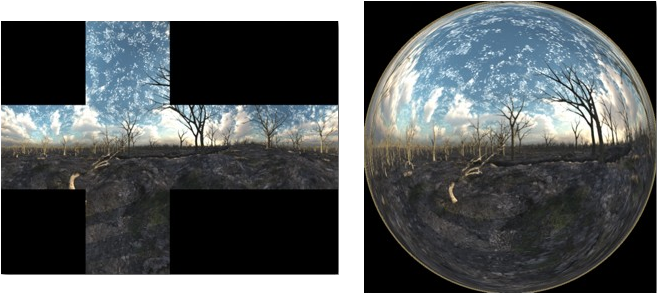
\includegraphics[width=1\linewidth]{images/chapter_lrl/lrl_envmapcubica.png}\hfill
 \caption[Env map di riflessione]{A sinistra una env map generata da una CubeCamera, a destra la stessa env map applicata su una sfera}
 \label{fig:lrl_envmapcubica}
\end{figure}

Nel presente lavoro di tesi le env-map vengono calcolate solamente in Three.js e non attraverso l’utilizzo di uno strumento esterno più potente come Blender.
Three.js infatti, oltre a permettere di creare env-map in modo semplice ed efficiente, ha permesso di diminuire notevolmente il numero di informazioni che Blender ed il tool di visualizzazione in Three.js devono scambiarsi. Informazioni che prevedono i dati di 6 immagini per ogni oggetto che riflette o rifrae, dati che diverrebbe enormi nel caso in cui nella scena venissero utilizzati decine di effetti di riflessioni/rifrazione. Il tipo di formato utilizzato per lo scambio dei dati verrà approfondito nel paragrafo \ref{sec:chapter_architettura_sistema_formato_scambio}.
\\
Come spiegato precedentemente è però necessario che il calcolo avvenga solamente quando l’ambiente creato risulta completo e fisso. Se così non fosse gli effetti di riflessione o rifrazione non proietterebbero le nuove modifiche dell’ ambiente.
Inoltre è importante che le env-map vengano calcolate su una scena in cui il processo di bake è già stato eseguito, in modo da ottenere anche la riflessione/rifrazione di luci ed ombre.
\\
\begin{figure}[htb]
 \centering
 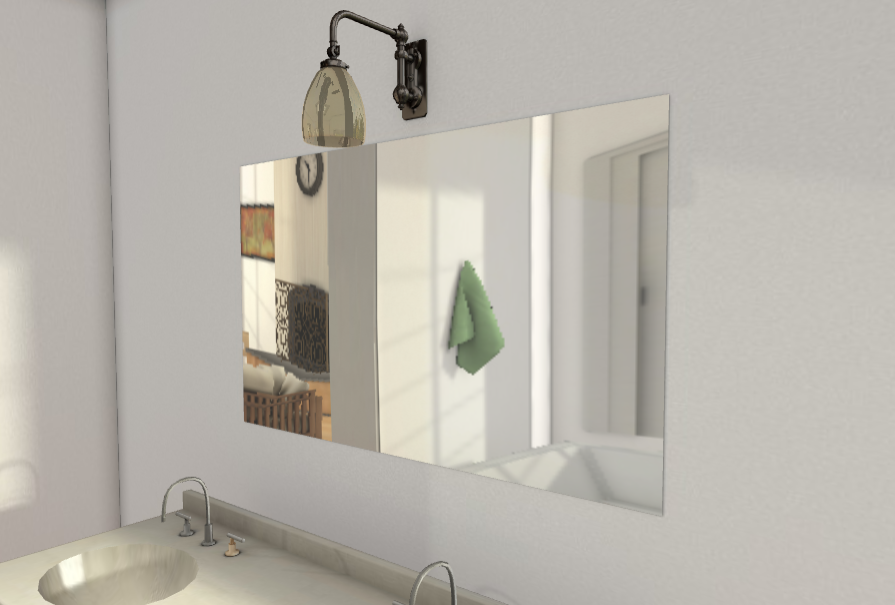
\includegraphics[width=1\linewidth]{images/chapter_lrl/lrl_envspecchio.png}\hfill
 \caption[Env map di riflessione]{Una env map di riflessione applicata su una superficie piano.}
 \label{fig:lrl_envspecchio}
\end{figure}

Nell’immagine è possibile notare come lo specchio rifletta l’ombra dell’ asciugamano verde e la luce proveniente dalla finestra. Questo sarebbe stato impossibile da realizzare se le env-map fossero state calcolate prima della procedura di bake in quanto gli effetti di luce non erano ancora stati calcolati ed applicati sull’ambiente renderizzato.
\\
Proprio per questo motivo la scena, dopo aver subito l’applicazione delle lightmap in Blender, viene  caricata sull’ editor online Three.js. Solamente dopo che il caricamento è stato completamente eseguito, nella vengono calcolate ed applicate le informazioni di riflessione e rifrazione (le envmap).
Questa proceduta ha permesso di ottenere realistici e credibili effetti di riflessione e rifrazione all’interno degli ambienti creati.
\\
Il funzionamento del servizio di bake e dell’editor three.js e di come essi interagiscono tra loro verrà chiarificato nei capitoli successivi.

